\subsection{Basics of sound}
Sound physically is propagation through a medium, a vibration which some things can produce and some things can pick up. The word sound can be used to describe both the propagation itself, but also the phenomenom we feel when our ears react to the propagation. Speakers, strings of a guitar and vocal chords (together with the lungs) are some of the things that can produce sound and microphones and membranes in ears are things that can pick up sound. The propagation will have a certain strength at some point in the medium it travels through, which can be measured. This allows us to model the pressure propagation, or the sound as a function of time. At time $t$ the pressure at some point can be denoted as $f(t)$. This function over time can also be called a signal.

% source: https://api.pageplace.de/preview/DT0400.9781292055152_A24617782/preview-9781292055152_A24617782.pdf The Science of Sound - Rossing, Moore, Wheeler

One of the simplest ways to generate a sound is connecting a speaker to a device that generates an analog current in the shape of a wave. The current moves an electromagnet which moves a membrane at the same frequency as the generator. This membrane displaces air at some rate which ears pick up as sound. A 440Hz wave, a signal that oscillates 440 times per second that is, will produce a sound wave of 440Hz \todo{this most likely needs a source}. An ear picks up this signal as what we call an A4 note. Ironically, the purity of the signal makes it sound harsh and it is noise in the signal that gives warmth and beauty to the note. This can be observed in figure \ref{fig:pianoWave} where the signal (sound made by an electric piano) largely matches a pure A4 (440Hz sinusoid) but not quite.

%https://eprints.hud.ac.uk/id/eprint/17816/1/Final_Thesis_-_November_2012.pdf

\begin{figure}[ht]
    \centering
    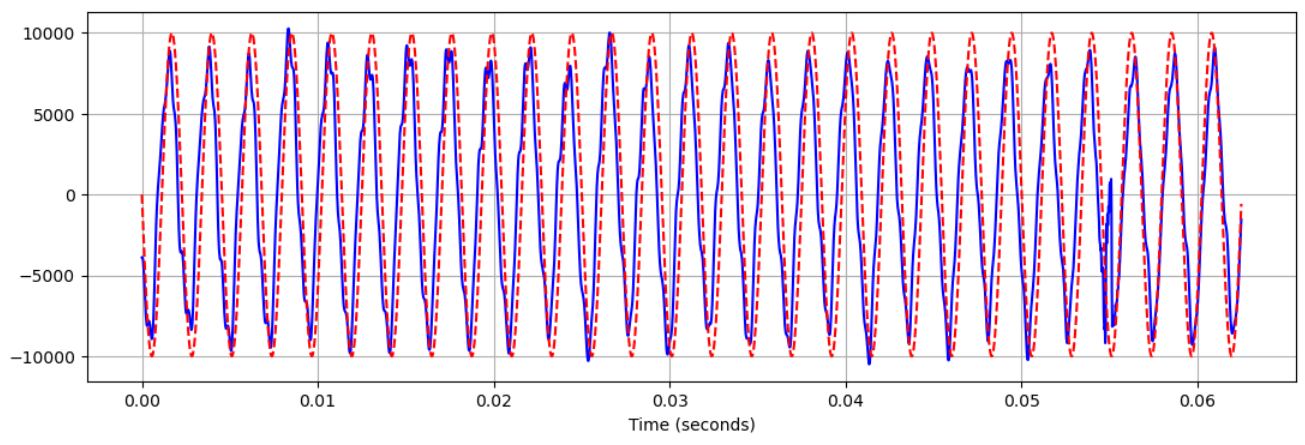
\includegraphics[width=\textwidth]{./images/piano_wave.png}
    \caption{A slice of the recording of a A4 note played on a Yamaha electric piano (blue solid). The signal contains a lot of irregularity but also clear regularity which becomes more evident when layering a pure A4 note on top (red dashed).\label{fig:pianoWave}}
\end{figure}

The characteristics of the sound being played becomes even more evident when it's converted to the frequency-domain through the FFT as shown in figure \ref{fig:pianoFreq}. It reveals that, not only is the sound definitely a A4 note due to the overwhelming amount of the 440Hz signal present in the sound, but also what other frequencies contribute to the sound of that piano.

\begin{figure}[ht]
    \centering
    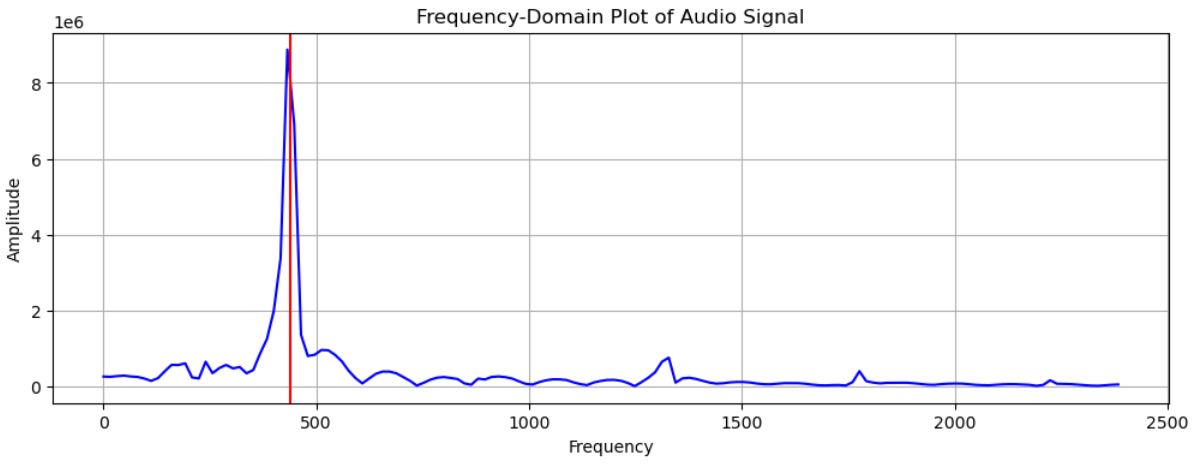
\includegraphics[width=\textwidth]{./images/piano_freq.png}
    \caption{The frequency-domain clearly reveals without any guesswork that the signal is a 440Hz signal with some sort of noise/disturbance. The red vertical line is placed at $x=440$ to show that the peak is the expected 440Hz frequency component.\label{fig:pianoFreq}}
\end{figure}

A human voice is even messier. 